\documentclass{exercise}

\institute{Lehrstuhl für Strömungslehre und Aerodynamisches Institut}
\title{Altklausur 2}
\author{Joshua Feld, 406718}
\course{Strömungsmechanik I}
\professor{Schröder}
\semester{Sommersemester 2022}
\program{CES (Bachelor)}

\begin{document}
    \maketitle


    \section*{Aufgabe 1}
    
    \begin{problem}
        Ein Ballon mit starrer Hülle ist vollständig mit einem Gas unbekannter Dichte gefüllt und hat unten eine Öffung zum Druckausgleich mit der Umgebung.
        Das Gewicht des Ballons ohne Gasfüllung beträgt \(G\).
        Vor dem Start wird der Ballon mit der Kraft \(F_s\) gehalten und steigt auf seine maximale Höhe \(z = H\), sobald er losgelassen wird.
        \begin{center}
            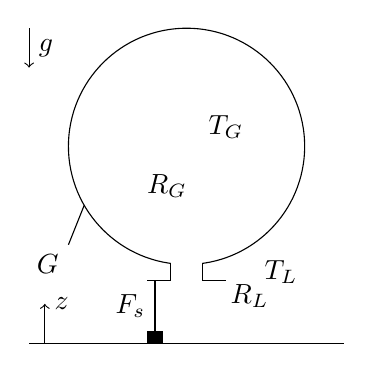
\begin{tikzpicture}
                \draw (0,2.5) circle (1.5cm);
                \fill[white] (-.2,1.2) rectangle (.2,.8);
                \draw (-.2,1) -- (-.2,.8) -- (-.5,.8);
                \draw (.2,1) -- (.2,.8) -- (.5,.8);
                \draw (-2,0) -- (2,0);
                \draw[->] (-1.8,0) -- (-1.8,.5) node[right] {\(z\)};
                \fill (-.5,0) rectangle (-.3,.15);
                \draw (-.4,.15) -- (-.4,.8) node[midway,left] {\(F_s\)};
                \draw[->] (-2,4) -- (-2,3.5) node[midway,right] {\(g\)};
                \draw (-1.5,1.25) node[below left] {\(G\)} -- (-1.3,1.75);
                \node at (-.25,2) {\(R_G\)};
                \node at (.5,2.75) {\(T_G\)};
                \node at (.8,.6) {\(R_L\)};
                \node at (1.2,.9) {\(T_L\)};
            \end{tikzpicture}
        \end{center}
        \begin{enumerate}
            \item Leiten Sie für eine isotherme Atmosphäre die barometrische Höhenformel her und geben Sie für das Gas im Ballon das Dichteverhältnis \(\frac{\rho_G\parentheses*{z = H}}{\rho_G\parentheses*{z = 0}}\) an.
            \item Ermitteln Sie die maximale Steighöhe \(H\) in isothermer Atmosphäre.
        \end{enumerate}
        Gegeben: \(G, F_s, g, R_L, T_L\)

        \emph{Hinweis:
        \begin{itemize}
            \item Für die isotherme Atmosphäre gilt \(T_L = T_G = \text{konst.}\)
            \item Luft und Gas dürfen als ideale Gase behandelt werden.
            \item Die Masse des unbekannten Gases darf nicht vernachlässigt werden.
            \item Überprüfen Sie Ihre Ergebnisse hinsichtlich der Plausibilität von Einheit und Vorzeichen.
        \end{itemize}}
    \end{problem}
    
    \subsection*{Lösung}
    \begin{enumerate}
        \item Die hydrostatische Grundgleichung \(\frac{\d p}{\d z} = -\rho g\) und das ideale Gasgesetz \(\rho = \frac{p}{RT}\) ergeben zusammen
        \[
            \frac{\d p}{\d z} = -\frac{pg}{RT}.
        \]
        Für eine isotherme Atmosphäre ergibt sich dann die barometrische Höhenformel zu
        \[
            \int_{p_0}^{p_1} = \ln\parentheses*{\frac{p_1}{p_0}} = -\frac{g}{RT}\int_{z_0}^{z_1}\d z = -\frac{g}{RT}\parentheses*{z_1 - z_0},
        \]
        bzw. mit \(z_1 - z_0 = H\)
        \[
            p\parentheses*{z = H} = p\parentheses*{z = 0}e^{-\frac{gH}{RT_L}}.
        \]
        Für einen offenen Ballon gilt \(p_L = p_G\), sodass
        \begin{align*}
            p_G\parentheses*{z = H} = \rho_G\parentheses*{z = H}R_G T_G \quad \text{und} \quad p_G\parentheses*{z = 0} = \rho_G\parentheses*{z = 0}R_G T_G,
        \end{align*}
        woraus
        \[
            \frac{\rho_G\parentheses*{z = H}}{\rho_G\parentheses*{z = 0}} = \frac{p_G\parentheses*{z = H}}{p_G\parentheses*{z = 0}} = \frac{p_L\parentheses*{z = H}}{p_L\parentheses*{z = 0}} = e^{-\frac{gH}{R_L T_L}}.
        \]
        \item Wir bestimmen zunächst die Auftriebskräfte am Boden und der Luft aus den entsprechenden Kräftegleichgewichten:
        \begin{align*}
            F_A\parentheses*{z = H} &= \rho_L\parentheses*{z = H}gV_B = G + G_{\text{Gas}}\parentheses*{z = H},\\
            F_A\parentheses*{z = 0} &= \rho_L\parentheses*{z = 0}gV_B = G + G_{\text{Gas}}\parentheses*{z = 0},
        \end{align*}
        mit \(G_{\text{Gas}}\parentheses*{z} = \frac{p_G\parentheses*{z}}{R_G T_G}gV_B\).
        Mit dem Ergebnis aus Teilaufgabe a) ergibt sich dann
        \[
            \rho_G\parentheses*{z = H} = \rho_G\parentheses*{z = 0}e^{-\frac{gH}{R_L T_L}} \quad \text{und} \quad \rho_L\parentheses*{z = H} = \rho_L\parentheses*{z = 0}e^{-\frac{gH}{R_L T_L}}
        \]
        und es folgt
        \[
            \rho_G\parentheses*{z = 0}gV_B = \rho_L\parentheses*{z = 0}V_Bg - G - F_s \iff \rho_G\parentheses*{z = 0} = \frac{\rho_L\parentheses*{z = 0}V_B g - G - F_s}{V_B g}.
        \]
        Einsetzen in das Kräftegleichgewicht liefert
        \begin{align*}
            \rho_L\parentheses*{z = 0}V_B ge^{-\frac{gH}{R_L T_L}} &= G + \frac{\rho_L\parentheses*{z = 0}V_B g - G - F_s}{V_B g}V_B ge^{-\frac{gH}{R_L T_L}}\\
            \iff \rho_L\parentheses*{z = 0}V_B ge^{-\frac{hH}{R_L T_L}} &= G + \parentheses*{\rho_L\parentheses*{z = 0}V_B g - G - F_s}^{-\frac{gH}{R_L T_L}}\\
            \iff 0 &= G - \parentheses*{G + F_s}e^{-\frac{gH}{R_L T_L}}\\
            \iff e^{-\frac{gH}{R_L T_L}} &= \frac{G}{G + F_s}\\
            \iff H &= \frac{R_L T_L}{g}\ln\parentheses*{1 + \frac{F_s}{G}}.
        \end{align*}
    \end{enumerate}


    \section*{Aufgabe 2}
    
    \begin{problem}
        Zwei oben offene Wasserbehälter haben beiden am Boden ein kleines Loch mit der Querschnittsfläche \(A_1\) (\(A_1 \ll R^2\)).
        Der erste Behälter hat die Form einer Kugel mit dem Radius \(R\), der zweite die Form eines Zylinders ebenfalls mit dem Radius \(R\).
        Beide Gefäße sind zum Zeitpunkt \(t = 0\) mit Wasser der Dichte \(\rho\) bis zu einer Höhe von \(\frac{3}{2}R\) gefüllt.
        \begin{center}
            \begin{tikzpicture}
                \draw (0,0) circle (2cm);
                \fill[white] (-.2,-2.2) rectangle (.2,-1.8);
                \draw (-.2,-2) -- (-.2,-2.375) node[below left] {\(A_1\)};
                \draw (.2,-2) -- (.2,-2.375);
                \fill[white] (-.2,2.2) rectangle (.2,1.8);
                \draw (-.2,1.8) -- (-.2,2.2);
                \draw (.2,1.8) -- (.2,2.2);
                \draw (1.5,-2) -- (3,-2);
                \draw[dashed] (0,2.5) -- (0,-2.5);
                \draw (-1.732,1) -- (1.732,1);
                \draw[dashed] (-1.732,-1) -- (2.25,-1);
                \draw[dashed] (-2.5,0) -- (2.5,0);
                \draw[<->] (2,-2) -- (2,-1) node[midway,right] {\(\frac{1}{2}R\)};
                \draw (2,1) -- (3,1);
                \draw[<->] (2.75,-2) -- (2.75,1) node[midway,right] {\(\frac{3}{2}R\)};
                \node at (2.5,2) {\(p_a\)};
                \draw[->] (0,0) -- (2,0) node[midway,above] {\(R\)};
                \draw (-.5,1) -- (-.6,1.2) -- (-.4,1.2) -- cycle;
                \draw[->] (-2,2) -- (-2,1.5) node[midway,right] {\(g\)};
                \begin{scope}[shift={(6,0)}]
                    \draw (-.2,2) -- (-2,2) -- (-2,-2) -- (-.2,-2) -- (-.2,-2.375) node[below left] {\(A_1\)};
                    \draw (-.2,2.2) -- (-.2,1.8);
                    \draw (.2,2) -- (2,2) -- (2,-2) -- (.2,-2) -- (.2,-2.375);
                    \draw (.2,2.2) -- (.2,1.8);
                    \draw (-2,1) -- (2,1);
                    \draw (-.5,1) -- (-.6,1.2) -- (-.4,1.2) -- cycle;
                    \draw[dashed] (0,2.5) -- (0,-2.5);
                    \draw (-1,1) -- (-1,-1.5);
                    \draw[->] (0,0) -- (2,0) node[midway,above] {\(R\)};
                    \draw[dashed] (-2,-1.5) -- (2,-1.5);
                    \draw (2.25,-2) -- (2.75,-2);
                    \draw[->] (2.5,-2) -- (2.5,-1.25) node[right] {\(z\)};
                \end{scope}
            \end{tikzpicture}
        \end{center}
        \begin{enumerate}
            \item Berechnen Sie die Zeit \(\Delta t\), in der die Spiegelhöhe im kugelförmigen Behälter um den Betrag \(R\) sinkt.
            \item Argumentieren Sie qualitativ, ob die Spiegelhöhendifferenz \(\Delta h\), die sich im zylindrischen Behälter in der selben Zeit \(\Delta t\) einstellt, größer, kleiner oder gleich ist, wie im kugelförmigen Behälter.
        \end{enumerate}
        Gegeben: \(A_1, \rho, g, R\)

        \emph{Hinweis:
        \begin{itemize}
            \item Die Strömung ist als quasistationär zu betrachten.
            \item Überprüfen Sie Ihre Ergebnisse hinsichtlich der Plausibilität von Einheit und Vorzeichen.
        \end{itemize}}
    \end{problem}

    \subsection*{Lösung}
    \begin{enumerate}
        \item\,
        \begin{center}
            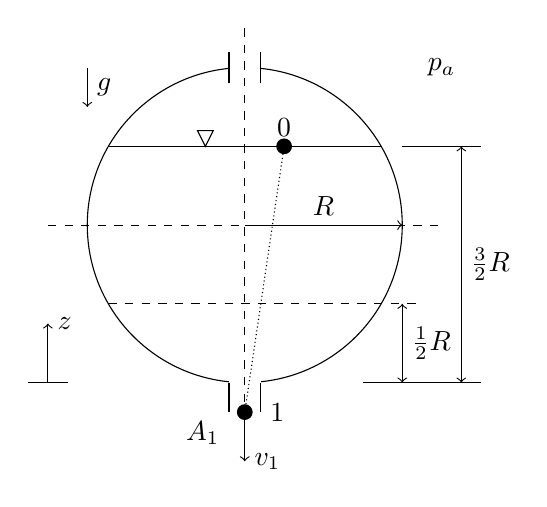
\begin{tikzpicture}
                \draw (0,0) circle (2cm);
                \fill[white] (-.2,-2.2) rectangle (.2,-1.8);
                \draw (-.2,-2) -- (-.2,-2.375) node[below left] {\(A_1\)};
                \draw (.2,-2) -- (.2,-2.375);
                \fill[white] (-.2,2.2) rectangle (.2,1.8);
                \draw (-.2,1.8) -- (-.2,2.2);
                \draw (.2,1.8) -- (.2,2.2);
                \draw (1.5,-2) -- (3,-2);
                \draw[dashed] (0,2.5) -- (0,-2.5);
                \draw (-1.732,1) -- (1.732,1);
                \draw[dashed] (-1.732,-1) -- (2.25,-1);
                \draw[dashed] (-2.5,0) -- (2.5,0);
                \draw[<->] (2,-2) -- (2,-1) node[midway,right] {\(\frac{1}{2}R\)};
                \draw (2,1) -- (3,1);
                \draw[<->] (2.75,-2) -- (2.75,1) node[midway,right] {\(\frac{3}{2}R\)};
                \node at (2.5,2) {\(p_a\)};
                \draw[->] (0,0) -- (2,0) node[midway,above] {\(R\)};
                \draw (-.5,1) -- (-.6,1.2) -- (-.4,1.2) -- cycle;
                \draw[->] (-2,2) -- (-2,1.5) node[midway,right] {\(g\)};
                \draw (-2.25,-2) -- (-2.75,-2);
                \draw[->] (-2.5,-2) -- (-2.5,-1.25) node[right] {\(z\)};
                \fill (.5,1) circle (1mm) node[above] {\(0\)};
                \fill (0,-2.375) circle (1mm);
                \node[anchor=west] at (.2,-2.375) {\(1\)};
                \draw[densely dotted] (.5,1) -- (0,-2.375);
                \draw[->] (0,-2.375) -- (0,-3) node[right] {\(v_1\)};
            \end{tikzpicture}
        \end{center}
        Die quasistationäre Bernoulli-Gleichung von \(0\) nach \(1\) liefert
        \[
            p_a + \frac{1}{2}\rho v_0^2 + \rho gz = p_a + \frac{1}{2}\rho v_1^2.
        \]
        Mit \(v_0 \ll v_1\), da \(A_1 \ll R^2\) ergibt sich die Torricelli-Gleichung
        \begin{equation}\label{eq:1}
            v_1 = \sqrt{2gz}.
        \end{equation}
        Aus der Kontinuitätsgleichung erhalten wir
        \begin{equation}\label{eq:2}
            v_1 A_1 = v\parentheses*{z}A\parentheses*{z} = -\frac{\d z}{\d t}A\parentheses*{z}.
        \end{equation}
        \begin{center}
            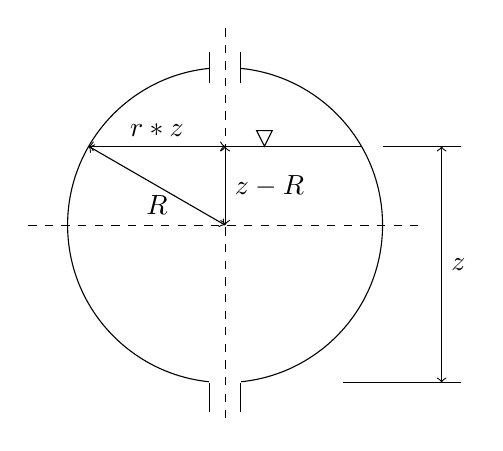
\begin{tikzpicture}
                \draw (0,0) circle (2cm);
                \fill[white] (-.2,-2.2) rectangle (.2,-1.8);
                \draw (-.2,-2) -- (-.2,-2.375);
                \draw (.2,-2) -- (.2,-2.375);
                \fill[white] (-.2,2.2) rectangle (.2,1.8);
                \draw (-.2,1.8) -- (-.2,2.2);
                \draw (.2,1.8) -- (.2,2.2);
                \draw (1.5,-2) -- (3,-2);
                \draw[dashed] (0,2.5) -- (0,-2.5);
                \draw (-1.732,1) -- (1.732,1);
                \draw[dashed] (-2.5,0) -- (2.5,0);
                \draw (2,1) -- (3,1);
                \draw[<->] (2.75,-2) -- (2.75,1) node[midway,right] {\(z\)};
                \draw (.5,1) -- (.6,1.2) -- (.4,1.2) -- cycle;
                \draw[<->] (0,0) -- (-1.732,1) node[midway,below] {\(R\)};
                \draw[<->] (0,1) -- (-1.732,1) node[midway,above] {\(r\parentheses*{z}\)};
                \draw[<->] (0,0) -- (0,1) node[midway,right] {\(z - R\)};
            \end{tikzpicture}
        \end{center}
        Für die Querschnittsfläche in Abhängigkeit von der aktuellen Füllstandshöhe \(z\) erhalten wir den Ausdruck
        \[
            A\parentheses*{z} = \pi r^2\parentheses*{z},
        \]
        wobei der Radius gegeben ist durch
        \[
            r^2\parentheses*{z} + \parentheses*{z - R}^2 = R^2 \iff r^2\parentheses*{z} = 2Rz - z^2,
        \]
        also insgesamt
        \begin{equation}\label{eq:3}
            A\parentheses*{z} = \pi\parentheses*{2Rz - z^2}.
        \end{equation}
        Setzen wir nun \eqref{eq:1} und \eqref{eq:3} in \eqref{eq:2} ein und formen um, so erhalten wir
        \begin{align*}
            \sqrt{2gz} A_1 &= -\frac{\d z}{\d t}\pi\parentheses*{2Rz - z^2}\\
            \iff \int_0^{\Delta t}\d t &= \int_{\frac{3}{2}R}^{\frac{1}{2}R}-\frac{\pi\parentheses*{2Rz - z^2}}{\sqrt{2gz}A_1}\d z\\
            \iff \Delta t &= \frac{\pi}{\sqrt{2g}A_1}\int_{\frac{3}{2}R}^{\frac{1}{2}R}\frac{z^2 - 2Rz}{\sqrt{z}}\d z\\
            &= \frac{\pi}{\sqrt{2g}A}\brackets*{\frac{2}{5}z^{\frac{5}{2}} - \frac{4}{3}Rz^{\frac{3}{2}}}_{\frac{3}{2}R}^{\frac{1}{2}R}\\
            &= \frac{2\pi R^{\frac{5}{2}}}{\sqrt{2g}A_1}\parentheses*{\frac{2}{3} \cdot \parentheses*{\parentheses*{\frac{3}{2}}^{\frac{3}{2}} - \parentheses*{\frac{1}{2}}^{\frac{3}{2}}} - \frac{1}{5} \cdot \parentheses*{\parentheses*{\frac{3}{2}}^{\frac{5}{2}} - \parentheses*{\frac{1}{2}}^{\frac{5}{2}}}}.
        \end{align*}
        \item Auch hier gilt die Kontinuitätsgleichung
        \[
            v_1 A_1 = -\frac{\d z}{\d t}A\parentheses*{z} \iff \d z = -\frac{v_1 A_1}{A\parentheses*{z}}\d t.
        \]
        Da der zylindrische Behälter eine größere Querschnittsfläche \(A_z\) als der kugelförmige Behälter hat, ist die Spiegelhöhenänderung im zylindrischen Behälter geringer, d.h. es gilt
        \[
            \left.\Delta h\right|_{\text{Zylinder}} < \left.\Delta h\right|_{\text{Kugel}}
        \]
        für das gleiche \(\Delta t\).
    \end{enumerate}


    \section*{Aufgabe 3}
    
    \begin{problem}
        Ein Strahlapparat, der von einem Gebläse angetrieben wird, saugt den Bypassstrom \(\dot{V}_2\) durch einen ringförmigen Einlauf aus der Umgebung an.
        \begin{center}
            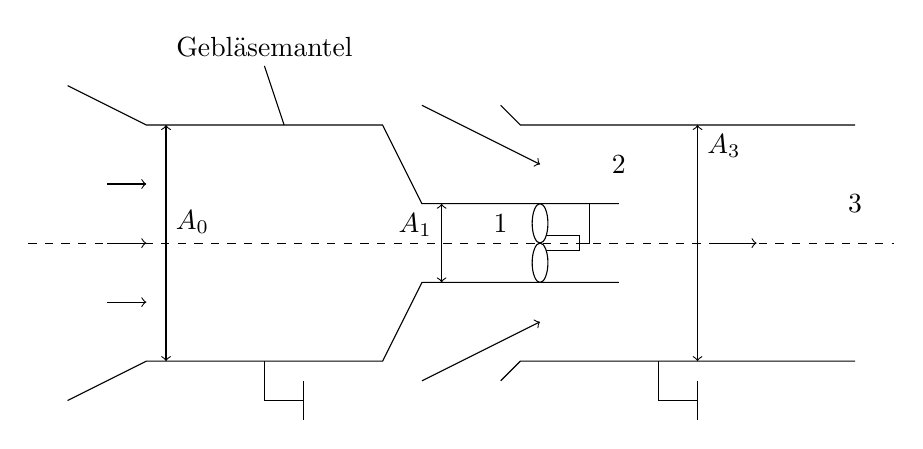
\begin{tikzpicture}
                \draw (0,2) -- (1,1.5) -- (4,1.5) -- (4.5,.5) -- (7,.5);
                \draw (0,-2) -- (1,-1.5) -- (4,-1.5) -- (4.5,-.5) -- (7,-.5);
                \draw (5.5,1.75) -- (5.75,1.5) -- (10,1.5);
                \draw (5.5,-1.75) -- (5.75,-1.5) -- (10,-1.5);
                \draw[dashed] (-.5,0) -- (10.5,0);
                \node at (5.5,.25) {\(1\)};
                \node at (7,1) {\(2\)};
                \node at (10,.5) {\(3\)};
                \draw (6,-.1) rectangle (6.5,.1);
                \draw (6.5,0) -- (6.625,0) -- (6.625,.5);
                \draw[fill=white] (6,.25) ellipse (1mm and 2.5mm);
                \draw[fill=white] (6,-.25) ellipse (1mm and 2.5mm);
                \draw[<->] (4.75,-.5) -- (4.75,.5) node[below left] {\(A_1\)};
                \draw[<->] (1.25,1.5) -- (1.25,-1.5) node[midway,above right] {\(A_0\)};
                \draw[->] (.5,.75) -- (1,.75);
                \draw[->] (.5,0) -- (1,0);
                \draw[->] (.5,-.75) -- (1,-.75);
                \draw[<->] (8,-1.5) -- (8,1.5) node[below right] {\(A_3\)};
                \draw[->] (8.25,0) -- (8.75,0);
                \draw (2.75,1.5) -- (2.5,2.25) node[above] {Gebläsemantel};
                \draw[->] (4.5,1.75) -- (6,1);
                \draw[->] (4.5,-1.75) -- (6,-1);
                \draw (2.5,-1.5) -- (2.5,-2) -- (3,-2);
                \draw (3,-1.75) -- (3,-2.25);
                \draw (7.5,-1.5) -- (7.5,-2) -- (8,-2);
                \draw (8,-1.75) -- (8,-2.25);
            \end{tikzpicture}
        \end{center}
        \begin{enumerate}
            \item Bestimmen Sie den statischen Druck im Querschnitt \(2\) und die Geschwindigkeiten in den Querschnitten \(1\) und \(3\).
            \item Wie groß ist die Haltekraft des Gebläsemantels unter der Annahme, dass die Querschnittsfläche des Bypassstromes deutlich größer ist als \(A_3\)?
            \item Berechnen Sie die Leistung, die dem Gebläse zugeführt werden muss.
        \end{enumerate}
        Gegeben: \(p_a, \rho, \dot{V}_2, A_1, \frac{A_3}{A_1} = \frac{3}{2}\)

        \emph{Hinweis:
        \begin{itemize}
            \item Die Strömung sei drall- und reibungsfrei.
            \item Überprüfen Sie Ihre Ergebnisse hinsichtlich der Plausibilität von Einheit und Vorzeichen.
        \end{itemize}}
    \end{problem}
    
    \subsection*{Lösung}
    \begin{enumerate}
        \item\,
        \begin{center}
            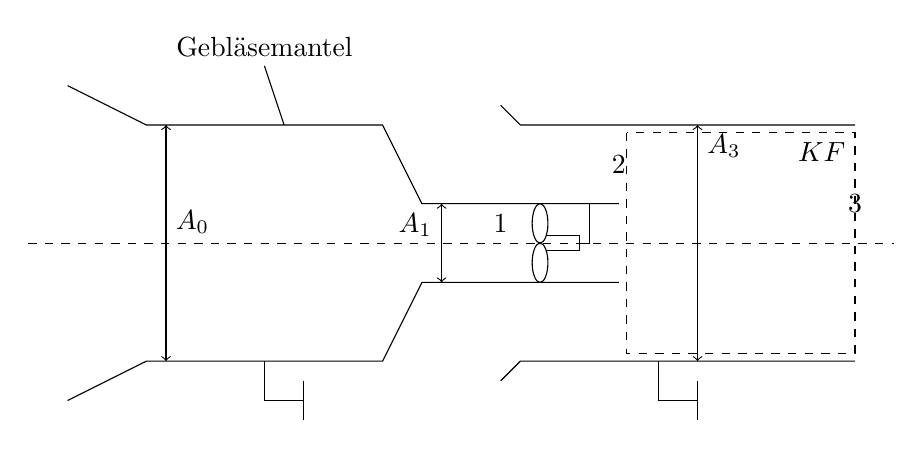
\begin{tikzpicture}
                \draw (0,2) -- (1,1.5) -- (4,1.5) -- (4.5,.5) -- (7,.5);
                \draw (0,-2) -- (1,-1.5) -- (4,-1.5) -- (4.5,-.5) -- (7,-.5);
                \draw (5.5,1.75) -- (5.75,1.5) -- (10,1.5);
                \draw (5.5,-1.75) -- (5.75,-1.5) -- (10,-1.5);
                \draw[dashed] (-.5,0) -- (10.5,0);
                \node at (5.5,.25) {\(1\)};
                \node at (7,1) {\(2\)};
                \node at (10,.5) {\(3\)};
                \draw (6,-.1) rectangle (6.5,.1);
                \draw (6.5,0) -- (6.625,0) -- (6.625,.5);
                \draw[fill=white] (6,.25) ellipse (1mm and 2.5mm);
                \draw[fill=white] (6,-.25) ellipse (1mm and 2.5mm);
                \draw[<->] (4.75,-.5) -- (4.75,.5) node[below left] {\(A_1\)};
                \draw[<->] (1.25,1.5) -- (1.25,-1.5) node[midway,above right] {\(A_0\)};
                \draw[<->] (8,-1.5) -- (8,1.5) node[below right] {\(A_3\)};
                \draw (2.75,1.5) -- (2.5,2.25) node[above] {Gebläsemantel};
                \draw (2.5,-1.5) -- (2.5,-2) -- (3,-2);
                \draw (3,-1.75) -- (3,-2.25);
                \draw (7.5,-1.5) -- (7.5,-2) -- (8,-2);
                \draw (8,-1.75) -- (8,-2.25);
                \draw[dashed] (7.1,1.4) rectangle (10,-1.4);
                \node[anchor=north east] at (10,1.4) {\(KF\)};
            \end{tikzpicture}
        \end{center}
        Die Bernoulli-Gleichung von \(\infty\) nach \(2\) ist
        \[
            p_a = p_2 + \frac{1}{2}v_2^2,
        \]
        wobei \(v_2 = \frac{\dot{V}_2}{A_2}\) und \(A_2 = A_3 - A_1 = \frac{1}{2}A_1\), d.h. die Bernoulli-Gleichung kann geschrieben werden als
        \begin{equation}\label{eq:4}
            p_2 = p_a - \frac{1}{2}\rho\parentheses*{\frac{2\dot{V}_2}{A_1}}^2 = p_a - 2\rho\frac{\dot{V}_2^2}{A_1^2}.
        \end{equation}
        Die Kontinuitätsgleichung ergibt sich hier zu
        \[
            \dot{V}_2 + v_1 A_1 = v_3 A_3 \iff \dot{V}_2 + v_1 A_1 = \frac{3}{2}v_3 A_1.
        \]
        Wir stellen nun noch eine Impulsbilanz auf
        \begin{align*}
            \underbrace{\frac{\d}{\d t}\iiint_V \rho u_j\d V}_{= 0\text{, da stationär}} + \iint_A \rho u_j u_i n_i\d A &= -\iint_A pn_j\d A + \underbrace{\iint_A \tau_{ij}n_i\d A}_{= 0\text{, da reibungsfrei}} + \underbrace{\iiint_V \rho k_j\d V}_{\substack{= 0\text{, da keine}\\\text{Volumenkräfte}}}\\
            \iff \iint_A \rho u_j u_i n_i\d A &= -\iint_A pn_j\d A
        \end{align*}
        und in \(x\)-Richtung gilt somit
        \begin{align*}
            \iint_A \rho u_x u_i n_i\d A &= -\iint pn_x\d A\\
            \iff \iint_{A_1}\rho v_1\parentheses*{-v_1}\d A + \iint_{A_2}\rho v_2\parentheses*{-v_2}\d A + \iint_{A_3}\rho v_3^2 \d A &= -\iint_{A_1}-p_2\d A - \iint_{A_2}-p_2\d A - \iint_{A_3}p_a\d A\\
            \iff -\rho A_1 v_1^2 - \rho A_2 v_2^2 + \rho A_3 v_3^2 &= p_2 A_1 + p_2 A_2 - p_a A_3\\
            \iff -\rho A_1 v_1^2 - \frac{1}{2}\rho A_1\parentheses*{\frac{2\dot{V}_2}{A_1}}^2 + \frac{3}{2}\rho A_1\parentheses*{\frac{2}{3}\frac{\dot{V}_2}{A_1} + \frac{2}{3}v_1}^2 &= p_2 A_1 + \frac{1}{2}p_2 A_1 - \frac{3}{2}p_a A_1\\
            \iff -\rho A_1 v_1^2 - 2\rho\frac{\dot{V}_2^2}{A_1} + \frac{2}{3}\rho A_1\parentheses*{\frac{\dot{V}_2^2}{A_1^2} + 2\frac{\dot{V}_2}{A_1}v_1 + v_1^2} &= -3\rho\frac{\dot{V}_2^2}{A_1}\\
            \iff -\rho A_1 v_1^2 - 2\rho\frac{\dot{V}_2^2}{A_1} + \frac{2}{3}\rho\frac{\dot{V}_2^2}{A_1} + \frac{4}{3}\rho\dot{V}_2 v_1 + \frac{2}{3}\rho A_1 v_1^2 &= -3\rho\frac{\dot{V}_2^2}{A_1}\\
            \iff -\frac{1}{3}\rho A_1 v_1^2 - \frac{4}{3}\rho\frac{\dot{V}_2^2}{A_1} + \frac{4}{3}\rho\dot{V}_2 v_1 &= -3\rho\frac{\dot{V}_2^2}{A_1}\\
            \iff v_1^2 - 4\frac{\dot{V}_2}{A_1}v_1 &= 5\frac{\dot{V}_2^2}{A_1^2}\\
            \iff \parentheses*{v_1 - 2\frac{\dot{V}_2}{A_1}}^2 - 4\frac{\dot{V}_2^2}{A_1^2} &= 5\frac{\dot{V}_2^2}{A_1^2}\\
            \iff v_1 - 2\frac{\dot{V}_2}{A_1} &= \pm 3\frac{\dot{V}_2}{A_1}
        \end{align*}
        und es folgen die Lösungen
        \[
            v_{1, 1} = 5\frac{\dot{V}_2}{A_1}, \quad v_{1, 2} = -\frac{\dot{V}_2}{A_1}.
        \]
        Die einzig physikalisch korrekte Lösung ist \(v_{1, 1}\), da bei \(v_{1, 2}\) der Strom in die andere Richtung laufen müsste, d.h. wir erhalten die Lösung
        \begin{equation}\label{eq:5}
            v_1 = 5\frac{\dot{V}_2}{A_1}.
        \end{equation}
        Für die zweite Geschwindigkeit folgt aus der Kontinuitätsgleichung sofort via Einsetzen von \eqref{eq:5}
        \[
            v_3 = 4\frac{\dot{V}_2}{A_1}.
        \]
        \item\,
        \begin{center}
            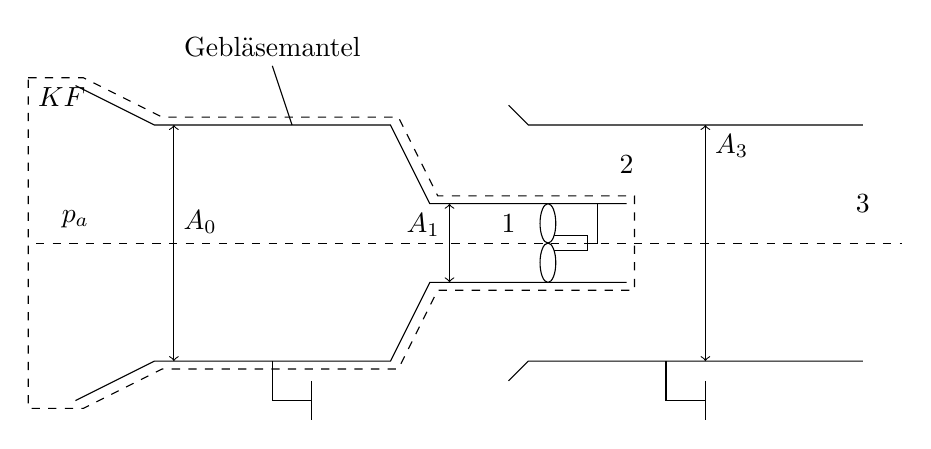
\begin{tikzpicture}
                \draw (0,2) -- (1,1.5) -- (4,1.5) -- (4.5,.5) -- (7,.5);
                \draw (0,-2) -- (1,-1.5) -- (4,-1.5) -- (4.5,-.5) -- (7,-.5);
                \draw (5.5,1.75) -- (5.75,1.5) -- (10,1.5);
                \draw (5.5,-1.75) -- (5.75,-1.5) -- (10,-1.5);
                \draw[dashed] (-.5,0) -- (10.5,0);
                \node at (5.5,.25) {\(1\)};
                \node at (7,1) {\(2\)};
                \node at (10,.5) {\(3\)};
                \draw (6,-.1) rectangle (6.5,.1);
                \draw (6.5,0) -- (6.625,0) -- (6.625,.5);
                \draw[fill=white] (6,.25) ellipse (1mm and 2.5mm);
                \draw[fill=white] (6,-.25) ellipse (1mm and 2.5mm);
                \draw[<->] (4.75,-.5) -- (4.75,.5) node[below left] {\(A_1\)};
                \draw[<->] (1.25,1.5) -- (1.25,-1.5) node[midway,above right] {\(A_0\)};
                \draw[<->] (8,-1.5) -- (8,1.5) node[below right] {\(A_3\)};
                \draw (2.75,1.5) -- (2.5,2.25) node[above] {Gebläsemantel};
                \draw (2.5,-1.5) -- (2.5,-2) -- (3,-2);
                \draw (3,-1.75) -- (3,-2.25);
                \draw (7.5,-1.5) -- (7.5,-2) -- (8,-2);
                \draw (8,-1.75) -- (8,-2.25);
                \draw[dashed] (-.6,2.1) node[below right] {\(KF\)} -- (.1,2.1) -- (1.1,1.6) -- (4.1,1.6) -- (4.6,.6) -- (7.1,.6) -- (7.1,-.6) -- (4.6,-.6) -- (4.1,-1.6) -- (1.1,-1.6) -- (.1,-2.1) -- (-.6,-2.1) -- cycle;
                \node at (0,.3) {\(p_a\)};
            \end{tikzpicture}
        \end{center}
        Wir arbeiten erneut mit einer Impulsbilanz
        \begin{align*}
            \underbrace{\frac{\d}{\d t}\iiint_V \rho u_j\d V}_{= 0\text{, da stationär}} + \iint_A \rho u_j u_i n_i\d A &= -\iint_A pn_j\d A + \underbrace{\iint_A \tau_{ij}n_i\d A}_{= 0\text{, da reibungsfrei}} + \underbrace{\iiint_V \rho k_j\d V}_{\substack{= 0\text{, da keine}\\\text{Volumenkräfte}}} + F_{j, \text{ext}}\\
            \iff \iint_A \rho u_j u_i n_i\d A &= -\iint_A pn_j\d A + F_{j, \text{ext}}
        \end{align*}
        Wieder gilt in \(x\)-Richtung
        \begin{align*}
            \iint_A \rho u_x u_i n_i\d A &= -\iint_A pn_x\d A + F_H\\
            \iff \iint_{A_1}\rho v_1^2\d A &= -\iint_{A_0}-p_a\d A - \iint_{A_0 - A_1}p_a\d A - \iint_{A_1}p_2\d A + F_H\\
            \iff \rho A_1 v_1^2 &= p_a A_0 - p_a\parentheses*{A_0 - A_1} - p_2 A_1 + F_H\\
            \iff \rho A_1 v_1^2 &= p_a A_1 - p_2 A_1 + F_H\\
            \iff F_H &= A_1\parentheses*{\rho v_1^2 - p_a + p_2}
        \end{align*}
        Setzen wir nun die Ergebnisse aus dem vorherigen Aufgabenteil ein, so erhalten wir schlussendlich
        \[
            F_H = 23\rho\frac{\dot{V}_2}{A_1}.
        \]
        \item Für die Gebläseleistung gilt
        \[
            P = \dot{V}\Delta p_0,
        \]
        mit \(\dot{V} = v_1 A_1\) und \(\Delta p_0 = p_2 - p_1\).
        Mit der Bernoulli-Gleichung von \(\infty\) nach \(1\) ergibt sich
        \[
            p_a = p_1 + \frac{1}{2}\rho v_1^2 \iff p_a - p_1 = \frac{1}{2}\rho v_1^2.
        \]
        Mit \(p_2 - p_a = -\frac{1}{2}\rho v_2^2\) aus \eqref{eq:4} ergibt sich
        \[
            p_2 - p_1 = p_2 - p_a + p_a - p_1 = \frac{1}{2}\parentheses*{v_1^2 - v_2^2} = \frac{21}{8}\rho v_2^2.
        \]
        Daraus folgt dann schlussendlich
        \[
            P = \frac{105}{16}\rho v_2^3 A_1 = \frac{105}{16}\rho\parentheses*{\frac{\dot{V}_2}{A_3 - A_1}}^2 A_1 = \frac{105}{2}\rho\frac{\dot{V}_2^3}{A_1^2}.
        \]
    \end{enumerate}


    \section*{Aufgabe 4}
    
    \begin{problem}
        In einem offenen Gerinne entsteht ein Wassersprung.
        \begin{center}
            \begin{tikzpicture}
                \draw[xscale=.1,domain=-6:6,smooth,variable=\x] plot ({\x},{1/(1+exp(-\x))});
                \draw (-.6,0) -- (-3,0);
                \draw (.6,1) -- (3,1);
                \draw (-3,-1.5) -- (3,-1.5);
                \node[anchor=north] at (-2,-1.5) {\(1\)};
                \node[anchor=north] at (2,-1.5) {\(2\)};
                \draw[<->] (-2,-1.5) -- (-2,0) node[midway,right] {\(h_1\)};
                \draw[<->] (2,-1.5) -- (2,1) node[midway,left] {\(h_2\)};
                \draw[->] (-2.5,1) -- (-2.5,.5) node[midway,right] {\(g\)};
                \draw[->] (-3.25,-.75) -- (-2.75,-.75) node[midway,above] {\(v_1\)};
                \draw[->] (2.75,-.25) -- (3.25,-.25) node[midway,above] {\(v_2\)};
                \draw[<->] (-3.75,-1) node[left] {\(y\)} -- (-3.75,-1.5) -- (-3.25,-1.5) node[above] {\(x\)};
            \end{tikzpicture}
        \end{center}
        \begin{enumerate}
            \item Skizzieren Sie sorgfältig den Verlauf der Energiehöhe entlang der \(x\)-Achse beim Übergang von Querschnitt \(1\) auf den Querschnitt \(2\).
            \item Die Spiegelhöhe \(h_2\) hinter dem Wassersprung beträgt \(h_2 = \frac{h_1}{2}\parentheses*{\sqrt{1 + 8Fr_1^2} - 1}\).
            Leiten Sie diesen Zusammenhang her.
            (Die Froude-Zahl \(Fr_1\) ist mit den Einströmgrößen zu bilden.)
            \item Bestimmen Sie den spezifischen Verlust an mechanischer Energie pro Zeiteinheit über den Wassersprung in Abhängigkeit der Froude-Zahl \(Fr_1\), dem auf die Kanalbreite bezogenen Volumenstrom \(q\), dem Verhältnis der Spiegelhöhen \(\frac{h_2}{h_1}\),der Dichte \(\rho\) und der Erdbeschleunigung \(g\).
            Benutzen Sie hierzu die Differenz der Energiehöhen vor und nach dem Wassersprung.
        \end{enumerate}
        \emph{Hinweis: Überprüfen Sie Ihre Ergebnisse hinsichtlich der Plausibilität von Einheit und Vorzeichen.}
    \end{problem}
    
    \subsection*{Lösung}
    \begin{enumerate}
        \item\,
        \begin{center}
            \begin{tikzpicture}
                \draw[<->] (-3,2.75) node[left] {\(H\)} -- (-3,0) -- (3,0) node[above] {\(x\)};
                \draw[xscale=.1,yscale=1.5,domain=-6:6,smooth,variable=\x] plot ({\x},{-1/(1+exp(-\x)) + 5/3});
                \draw (-2,.1) -- (-2,-.1) node[below] {\(1\)};
                \draw (2,.1) -- (2,-.1) node[below] {\(2\)};
                \draw (-3,2.5) -- (-.6,2.5);
                \draw (.6,1) -- (3,1);
                \draw[|<->] (2,2.5) -- (2,1) node[midway,right] {\(\Delta H\)};
            \end{tikzpicture}
        \end{center}
        \item\,
        \begin{center}
            \begin{tikzpicture}
                \draw[xscale=.1,domain=-6:6,smooth,variable=\x] plot ({\x},{1/(1+exp(-\x))});
                \draw (-.6,0) -- (-3,0);
                \draw (.6,1) -- (3,1);
                \draw (-3,-1.5) -- (3,-1.5);
                \node[anchor=north] at (-2,-1.5) {\(1\)};
                \node[anchor=north] at (2,-1.5) {\(2\)};
                \draw[<->] (-2,-1.5) -- (-2,0) node[midway,right] {\(h_1\)};
                \draw[<->] (2,-1.5) -- (2,1) node[midway,left] {\(h_2\)};
                \draw[->] (-2.5,1) -- (-2.5,.5) node[midway,right] {\(g\)};
                \draw[->] (-3.25,-.75) -- (-2.75,-.75) node[midway,above] {\(v_1\)};
                \draw[->] (2.75,-.25) -- (3.25,-.25) node[midway,above] {\(v_2\)};
                \draw[<->] (-3.75,-1) node[left] {\(y\)} -- (-3.75,-1.5) -- (-3.25,-1.5) node[above] {\(x\)};
                \draw[dashed] (-2.9,-1.4) rectangle (2.9,1.9);
                \node[anchor=north west] at (-2.9,1.9) {\(KF\)};
            \end{tikzpicture}
        \end{center}
        Für die Froude-Zahl gilt allgemein
        \[
            Fr = \frac{v}{\sqrt{gz}},
        \]
        d.h. wir erhalten hier
        \[
            Fr_1 = \frac{v_1}{\sqrt{gh_1}}.
        \]
        Sei \(B\) die Breite des Gerinnes.
        Aus der Kontinuitätsgleichung folgt
        \[
            \rho v_1 h_1 B = \rho v_2 h_2 B \iff v_1 h_1 = v_2 h_2.
        \]
        Wir stellen nun eine Impulsbilanzgleichung auf:
        \begin{align*}
            \underbrace{\frac{\d}{\d t}\iiint_V \rho u_j\d V}_{= 0\text{, da stationär}} + \iint_A \rho u_j u_i n_i\d A &= -\iint_A pn_j\d A + \underbrace{\iint_A \tau_{ij}n_i\d A}_{= 0\text{, da reibungsfrei}} + \iiint_V \rho k_j\d V\\
            \iff \iint_A \rho u_j u_i n_i\d A &= -\iint_A pn_j\d A + \iiint_V \rho k_j\d V.
        \end{align*}
        In \(x\)-Richtung ergibt sich
        \begin{align*}
            \iint_A \rho u_x u_i n_i\d A &= -\iint_A pn_x\d A + \underbrace{\iiint_V \rho k_x\d V}_{\substack{= 0\text{, da keine Volumen-}\\\text{kraft in }x\text{-Richtung}}}\\
            \iff \iint_A \rho u_x u_i n_i\d A &= -\iint_A pn_x\d A\\
            \iff -h_1 B\rho v_1^2 + h_2 B\rho v_2^2 &= B\int_0^{h_1}\parentheses*{p_a + \rho g\parentheses*{h_1 - y}}\d y + B\parentheses*{h_2 - h_1}p_a - B\int_0^{h_2}\parentheses*{p_a + \rho g\parentheses*{h_2 - y}}\d y\\
            \iff -h_1 B\rho v_1^2 + h_2 B\rho v_2^2 + Bp_a\parentheses*{h_1 - h_2} &= B\brackets*{p_a y + \rho g\parentheses*{h_1 y - \frac{1}{2}y^2}}_0^{h_1} - B\brackets*{p_a y + \rho g\parentheses*{h_2 y - \frac{1}{2}y^2}}_0^{h_2}\\
            \iff -h_1 \rho v_1^2 + h_2 v_2^2 + p_a\parentheses*{h_1 - h_2} &= p_a h_1 + \rho g\parentheses*{h_1^2 - \frac{1}{2}h_1^2} - \parentheses*{p_a h_2 + \rho g\parentheses*{h_2^2 - \frac{1}{2}h_2^2}}\\
            \iff -h_1 v_1^2 + \frac{h_1^2}{h_2}v_1^2 &= \frac{1}{2}g\parentheses*{h_1 - h_2}\parentheses*{h_1 + h_2}\\
            \iff \frac{h_1}{h_2}v_1^2\parentheses*{h_1 - h_2} &= \frac{1}{2}g\parentheses*{h_1 - h_2}\parentheses*{h_1 + h_2}\\
            \iff \frac{h_1}{h_2}v_1^2 &= \frac{1}{2}g\parentheses*{h_1 + h_2}\\
            \iff \frac{h_1^2}{h_2}\frac{v_1^2}{gh_1} &= \frac{h_1 + h_2}{2}\\
            \iff \frac{h_1^2}{h_2}Fr^2 &= \frac{h_1 + h_2}{2}\\
            \iff h_2^2 + h_1 h_2 &= 2Fr_1^2 h_1^2\\
            \iff \parentheses*{h_2 + \frac{1}{2}h_1}^2 &= h_1^2\parentheses*{\frac{1}{4} + 2Fr_1^2}\\
            \iff h_2 &= \frac{h_1}{2}\parentheses*{\sqrt{1 + 8Fr_1^2} - 1}.
        \end{align*}
        \item Die Verlustleistung \(P\) lässt sich angeben als
        \[
            P = q\Delta p_0 = \rho g\Delta Hq.
        \]
        Wir stellen nun die Energiegleichung auf und lösten diese nach dem Energiehöhenunterschied \(\Delta H\) auf:
        \begin{align*}
            h_1 + \frac{v_1^2}{2g} &= h_2 + \frac{v_1^2}{2g}\frac{h_1^2}{h_2^2} + \Delta H\\
            \iff h_2 - h_1 + \Delta H &= \frac{v_1^2}{2g}\parentheses*{1 - \parentheses*{\frac{h_1}{h_2}}^2}\\
            \iff \frac{h_2}{h_1} - 1 + \frac{\Delta H}{h_1} &= \frac{Fr_1^2}{2}\parentheses*{1 - \parentheses*{\frac{h_1}{h_2}}^2}\\
            \iff \Delta H &= h_1\parentheses*{1 - \frac{h_2}{h_1} + \frac{Fr_1^2}{2}\parentheses*{1 - \parentheses*{\frac{h_1}{h_2}}^2}}.
        \end{align*}
        Daraus folgt dann schlussendlich für die Verlustleistung
        \[
            P = \rho gqh_1\parentheses*{1 - \frac{h_2}{h_1} + \frac{Fr_1^2}{2}\parentheses*{1 - \parentheses*{\frac{h_1}{h_2}}^2}}.
        \]
    \end{enumerate}


    \section*{Aufgabe 5}
    
    \begin{problem}
        In einer ausgebildeten Rohrströmung befindet sich auf der Achse des kreisförmigen Rohres bis zum Radius \(R_1\) Öl und im äußeren Teil bis zur Rohrwnad (Radius \(R_2\)) Wasser.
        Der Druck fällt über die Länge \(L\) um den Wert \(\Delta p\) ab.
        \begin{center}
            \begin{tikzpicture}
                \draw (-3,2) -- (3,2);
                \draw (-2.5,1) -- (2.5,1);
                \draw[dashed] (-3.5,0) -- (3.5,0);
                \draw (-2.5,-1) -- (2.5,-1);
                \draw (-3,-2) -- (3,-2);
                \draw[->] (-3,0) -- (-3,2) node[midway,left] {\(R_2\)};
                \draw[->] (-2.5,0) -- (-2.5,1) node[midway,left] {\(R_1\)};
                \draw[<->] (-4.25,.5) node[left] {\(r\)} -- (-4.25,0) -- (-3.75,0) node[above] {\(x\)};
                \draw (-2.5,1.75) -- (-2.5,2.75) -- (2.5,2.75) -- (2.5,1.75);
                \draw[fill=white] (0,2.75) circle (3mm);
                \node at (0,2.75) {\(\Delta p\)};
                \draw[<->] (-2.5,1.875) -- (2.5,1.875) node[midway,below] {\(L\)};
                \node at (-1,1.5) {\(\eta_W\)};
                \node at (-.25,.5) {\(\eta_{\text{Öl}}\)};
                \node at (-1,-1.5) {\(\eta_W\)};
                \draw (-2.2,.75) circle (.5mm);
                \draw (-2.1,-.6) circle (.5mm);
                \draw (-2,.5) circle (.5mm);
                \draw (-1.9,.2) circle (.5mm);
                \draw (-1.8,-.3) circle (.5mm);
                \draw (-1.7,.9) circle (.5mm);
                \draw (-1.6,-.8) circle (.5mm);
                \draw (-1.5,.56) circle (.5mm);
                \draw (-1.4,.2) circle (.5mm);
                \draw (-1.3,.88) circle (.5mm);
                \draw (-1.2,-.6) circle (.5mm);
                \draw (-1.1,-.3) circle (.5mm);
                \draw (-1,.4) circle (.5mm);
                \draw (-.9,-.95) circle (.5mm);
                \draw (-.8,.24) circle (.5mm);
                \draw (-.7,-.7) circle (.5mm);
                \draw (-.6,.75) circle (.5mm);
                \draw (-.5,.4) circle (.5mm);
                \draw (-.4,-.33) circle (.5mm);
                \draw (-.3,.3) circle (.5mm);
                \draw (-.1,-.6) circle (.5mm);
                \draw (0,.1) circle (.5mm);
                \begin{scope}[shift={(2.3,0)}]
                    \draw (-2.2,.75) circle (.5mm);
                    \draw (-2.1,-.6) circle (.5mm);
                    \draw (-2,.5) circle (.5mm);
                    \draw (-1.9,.2) circle (.5mm);
                    \draw (-1.8,-.3) circle (.5mm);
                    \draw (-1.7,.9) circle (.5mm);
                    \draw (-1.6,-.8) circle (.5mm);
                    \draw (-1.5,.56) circle (.5mm);
                    \draw (-1.4,.2) circle (.5mm);
                    \draw (-1.3,.88) circle (.5mm);
                    \draw (-1.2,-.6) circle (.5mm);
                    \draw (-1.1,-.3) circle (.5mm);
                    \draw (-1,.4) circle (.5mm);
                    \draw (-.9,-.95) circle (.5mm);
                    \draw (-.8,.24) circle (.5mm);
                    \draw (-.7,-.7) circle (.5mm);
                    \draw (-.6,.75) circle (.5mm);
                    \draw (-.5,.4) circle (.5mm);
                    \draw (-.4,-.33) circle (.5mm);
                    \draw (-.3,.3) circle (.5mm);
                    \draw (-.2,.5) circle (.5mm);
                    \draw (-.1,-.6) circle (.5mm);
                \end{scope}
            \end{tikzpicture}
        \end{center}
        \begin{enumerate}
            \item Formulieren Sie das Kräftegleichgewicht in radialer und axialer Richtung, leiten Sie die Schubspannungsverteilung her und skizzieren Sie diese sorgfältig.
            \item Ermitteln Sie die Geschwindigkeitsverteilung und skizzieren Sie diese sorgfältig.
        \end{enumerate}
        Gegeben: \(\eta_W, \eta_{\text{Öl}}, \eta_{\text{Öl}} > \eta_W, \Delta p, L, R_1, R_2\)

        \emph{Hinweis:
        \begin{itemize}
            \item Öl und Wasser können als Newtonsches Fluid betrachtet werden.
            \item Der Einfluss der Gravitation kann vernachlässigt werden.
            \item Öl und Wasser vermischen sich nicht.
            \item Überprüfen Sie Ihre Ergebnisse hinsichtlich der Plausibilität von Einheit und Vorzeichen.
        \end{itemize}}
    \end{problem}
    
    \subsection*{Lösung}
    \begin{enumerate}
        \item\,
        \begin{center}
            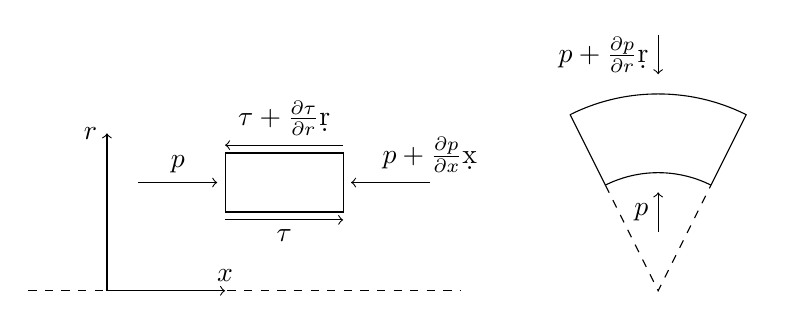
\begin{tikzpicture}
                \draw[<->] (0,2) node[left] {\(r\)} -- (0,0) -- (1.5,0) node[above] {\(x\)};
                \draw[dashed] (-1,0) -- (4.5,0);
                \draw (1.5,1) rectangle (3,1.75);
                \draw[->] (1.5,.9) -- (3,.9) node[midway,below] {\(\tau\)};
                \draw[->] (3,1.85) -- (1.5,1.85) node[midway,above] {\(\tau + \frac{\partial\tau}{\partial r}\d r\)};
                \draw[->] (.4,1.375) -- (1.4,1.375) node[midway,above] {\(p\)};
                \draw[->] (4.1,1.375) node[above] {\(p + \frac{\partial p}{\partial x}\d x\)} -- (3.1,1.375);
                \begin{scope}[shift={(7,0)}]
                    \begin{scope}
                        \clip (0,0) -- (-1.5,3) -- (1.5,3) -- cycle;
                        \draw (0,0) circle (1.5cm);
                        \draw (0,0) circle (2.5cm);
                    \end{scope}
                    \draw[dashed] (-.67,1.34) -- (0,0) -- (.67,1.34);
                    \draw (-.67,1.34) -- (-1.12,2.24);
                    \draw (.67,1.34) -- (1.12,2.24);
                    \draw[->] (0,.75) -- (0,1.25) node[midway,left] {\(p\)};
                    \draw[->] (0,3.25) -- (0,2.75) node[midway,left] {\(p + \frac{\partial p}{\partial r}\d r\)};
                \end{scope}
            \end{tikzpicture}
        \end{center}
        Wir stellen nun zunächst das Kräftegleichgewicht in axialer Richtung auf
        \begin{align*}
            2p\pi r\d r + 2\tau \pi r\d x - 2\parentheses*{p + \frac{\partial p}{\partial x}\d x}\pi r\d r - 2\parentheses*{\tau + \frac{\partial\tau}{\partial r}\d r}\pi\d x\parentheses*{r + \d r} &= 0\\
            \iff -2\pi \parentheses*{r\frac{\partial p}{\partial x}\d x\d r + \tau\d r\d x + r\frac{\partial\tau}{\partial r}\d r\d x + \frac{\partial\tau}{\partial r}\d r^2 \d x} &= 0\\
            \iff \frac{\partial p}{\partial x} + \frac{\tau}{r} + \frac{\partial\tau}{\partial r} + \underbrace{\frac{1}{r}\frac{\partial\tau}{\partial r}\d r}_{= 0\text{, vernachlässigbar}} &= 0\\
            \iff \frac{\partial p}{\partial x} = -\frac{\partial\tau}{\partial r} - \frac{\tau}{r} = -\frac{1}{r}\frac{\partial}{\partial r}\parentheses*{r\tau}.
        \end{align*}
        In radialer Richtung ergibt sich das Kräftegleichgewicht zu
        \begin{align*}
            pr\d\varphi - \parentheses*{p + \frac{\partial p}{\partial r}}\parentheses*{r + \d r}\d\varphi + 2\parentheses*{p + \frac{\partial p}{\partial r}\frac{\d r}{2}}\frac{\d\varphi}{2}\d r &= 0\\
            \iff -\frac{\partial p}{\partial r}r\d r\d\varphi - \frac{1}{2}\frac{\partial p}{\partial r}\d r^2 \d\varphi &= 0\\
            \iff \frac{\partial p}{\partial r} + \underbrace{\frac{1}{2r}\frac{\partial p}{\partial r}\d r}_{= 0\text{, vernachlässigbar}} &= 0\\
            \iff \frac{\partial p}{\partial r} &= 0
        \end{align*}
        Wir können nun also die partielle Ableitung aus dem Kräftegleichgewicht in axialer Richtung als totale Ableitung schreiben, da \(p\) offensichtlich unabhängig von \(r\) ist.
        Da diese totale Ableitung keine Abhängigkeit von \(x\) aufweist, wissen wir, dass der Druckverlauf in \(x\)-Richtung zudem linear ist und es gilt
        \[
            \frac{\d p}{\d x} = -\frac{1}{r}\frac{\partial}{\partial r}\parentheses*{\tau r} = -\frac{\Delta p}{L} \iff \frac{\partial}{\partial r}\parentheses*{\tau r} = \Delta p\frac{r}{L} \iff \tau r = \Delta p\frac{r^2}{2L} + c,
        \]
        woraus
        \[
            \tau = \Delta p\frac{r}{2L} + \frac{c}{r}.
        \]
        folgt.
        Für eine ausgebildete Rohrströmung wissen wir, dass gerade der Hochpunkt des Geschwindigkeitsprofils genau auf der Rotationsachse liegt und dementsprechend die Schubspannung dort gleich Null sein muss.
        Daraus können wir unsere Integrationskonstante \(c\) wie folgt bestimmen:
        \[
            \lim_{r \to 0}\tau \stackrel{!}{=} 0 \iff \lim_{r \to 0}\parentheses*{\Delta p\frac{r}{2L} + \frac{c}{r}} = 0 \implies c = 0.
        \]
        Somit erhalten wir für unser Schubspannungsprofil
        \[
            \tau\parentheses*{r} = \Delta p\frac{r}{2L}.
        \]
        Graphisch dargestellt sieht dieses Profil wie folgend skizziert aus:
        \begin{center}
            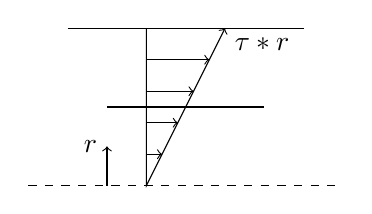
\begin{tikzpicture}
                \draw[dashed] (0,0) -- (4,0);
                \draw (1,1) -- (3,1);
                \draw (.5,2) -- (3.5,2);
                \draw[->] (1.5,2) -- (1.5,0) -- (2.5,2) node[below right] {\(\tau\parentheses*{r} \)};
                \draw[->] (1.5,.4) -- (1.7,.4);
                \draw[->] (1.5,.8) -- (1.9,.8);
                \draw[->] (1.5,1.2) -- (2.1,1.2);
                \draw[->] (1.5,1.6) -- (2.3,1.6);
                \draw[->] (1,0) -- (1,.5) node[left] {\(r\)};
            \end{tikzpicture}
        \end{center}
        \item Wir verwenden nun das Newtonsche Reibungsgesetz, da, nach dem gegebenen Hinweis, Öl und Wasser als Newtonsche Fluide betrachtet werden können, d.h. es gilt
        \[
            \tau = -\eta\frac{\d u}{\d r} = \Delta p\frac{r}{2L}.
        \]
        Es gilt also
        \[
            -\eta_{\parentheses*{\cdot}}\frac{\d u_{\parentheses*{\cdot}}}{\d r} = \Delta p\frac{r}{2L} \iff \frac{\d u_{\parentheses*{\cdot}}}{\d r} = -\frac{\Delta p}{\eta_{\parentheses*{\cdot}}}\frac{r}{2L} \iff u_{\parentheses*{\cdot}} = -\frac{\Delta p}{\eta_{\parentheses*{\cdot}}}\frac{r^2}{4L} + c_{\parentheses*{\cdot}}.
        \]
        Explizit für die beiden Komponenten aufgeschrieben erhalten wir
        \begin{align*}
            u_W &= -\frac{\Delta p}{\eta_W}\frac{r^2}{4L} + c_W,\\
            u_{\text{Öl}} &= -\frac{\Delta p}{\eta_{\text{Öl}}}\frac{r^2}{4L} + c_{\text{Öl}}.
        \end{align*}
        Wir wissen, dass an der Wand die Haftbedingung gilt und es keinen Geschwindigkeitssprung beim Übergang zwischen den beiden Phasen gibt, d.h. wir erhalten die folgenden zwei Bedingungen mit denen wir dann die Integrationskonstanten \(c_W\) und \(c_{\text{Öl}}\) bestimmen können
        \[
            u_W\parentheses*{r = R_2} = 0, \quad u_W\parentheses*{r = R_1} = u_{\text{Öl}}\parentheses*{r = R_1}.
        \]
        Aus der Haftbedingung folgt
        \[
            -\frac{\Delta p}{\eta_W}\frac{R_2^2}{4L} + c_W = 0 \iff c_W = \frac{\Delta p}{\eta_W}\frac{R_2^2}{4L} \implies u_W\parentheses*{r} = -\frac{\Delta p}{4\eta_W L}\parentheses*{R_2^2 - r^2}
        \]
        Aus der Übergangsbedingung folgt
        \[
            -\frac{\Delta p}{\eta_{\text{Öl}}}\frac{R_1^2}{4L} + c_{\text{Öl}} = -\frac{\Delta p}{4\eta_W L}\parentheses*{R_2^2 - R_1^2} \iff c_{\text{Öl}} = -\frac{\Delta p}{4\eta_W L}\parentheses*{R_2^2 - R_1^2} + \frac{\Delta p}{\eta_{\text{Öl}}}\frac{R_1^2}{4L}
        \]
        und somit
        \[
            u_{\text{Öl}}\parentheses*{r} = \frac{\Delta p}{4\eta_{\text{Öl}}L}\parentheses*{R_1^2 - r^2} - \frac{\Delta p}{4\eta_W L}\parentheses*{R_2^2 - R_1^2}.
        \]
        Insgesamt gilt somit für das Geschwindigkeitsprofil
        \[
            u\parentheses*{r} = \begin{cases}
                \frac{\Delta p}{4\eta_{\text{Öl}}L}\parentheses*{R_1^2 - r^2} - \frac{\Delta p}{4\eta_W L}\parentheses*{R_2^2 - R_1^2}, & \text{falls }0 \le r < R_1,\\
                -\frac{\Delta p}{4\eta_W L}\parentheses*{R_2^2 - r^2}, & \text{falls }R_1 \le r \le R_2.
            \end{cases}
        \]
        Graphisch ergibt sich das folgende Erscheinungsbild:
        \begin{center}
            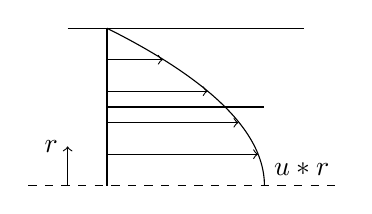
\begin{tikzpicture}
                \draw[dashed] (0,0) -- (4,0);
                \draw (1,1) -- (3,1);
                \draw (.5,2) -- (3.5,2);
                \draw[domain=0:2,smooth,variable=\y] plot ({-1/2*(\y*\y - 6)}, {\y});
                \draw (1,0) -- (1,2);
                \draw[->] (1,.4) -- (2.92,.4);
                \draw[->] (1,.8) -- (2.67,.8);
                \draw[->] (1,1.2) -- (2.28,1.2);
                \draw[->] (1,1.6) -- (1.71,1.6);
                \draw[->] (.5,0) -- (.5,.5) node[left] {\(r\)};
                \node[anchor=south west] at (3,0) {\(u\parentheses*{r}\)};
            \end{tikzpicture}
        \end{center}
    \end{enumerate}


    \section*{Aufgabe 6}
    
    \begin{problem}
        \begin{enumerate}
            \item Was versteht man unter einer Couette-Strömung?
            \item Formulieren Sie die allgemeine Gleichung für den Impulsmomentensatz einer stationären Strömung.
            \item Erklären Sie die Eulersche und Lagrangesche Form der Strömungsbeschreibung.
            Wo liegen bei diesen Ansätzen die Unterschiede?
            \item Drücken Sie die turbulente Schubspannung anhand der Prandtlschen Mischungswehhypothese aus.
            Definieren Sie ebenfalls, in Anlehnung an den Boussinesq-Ansatz, die zugehörige turbulente Zähigkeit.
            \item Was beschreibt das universelle logarithmische Wandgesetz?
            \item Nennen Sie zwei Eigenschaften, durch die sich die viskose Unterschicht auszeichnet.
        \end{enumerate}
    \end{problem}
    
    \subsection*{Lösung}
    \begin{enumerate}
        \item Unter eine Couette-Strömung versteht man eine stationäre Strömung zwischen zwei unendlichen Platten, die relativ zueunander verschoben werden.
        \item
        \[
            \sum\vec{M} = \int_{KF}\parentheses*{\vec{r} \times \vec{v}}\rho\parentheses*{\vec{v} \cdot \vec{n}}\d A.
        \]
        \item Bei dem Lagrange-Ansatz wird die Bewegung der einzelnen Fluidpartikel verfolgt und hieraus die Änderungen der Fluideigenschaften bestimmt, die mit diesen Teilchen verbunden sind.
        Die Eulersche Beschreibung hingegen verwendet das Feldkonzept.
        Es werden zu einem gewissen Zeitpunkt die Variablen des Strömungsfeldes wie Dichte, Druck, Geschwindigkeit oder Beschleunigung als Funktion der räumlichen Koordinaten \(x\), \(y\) und \(z\) dargestellt.
        \item Die Prandtlsche Mischungsweghypothese ist
        \[
            \tau_t = \rho l^2 \absolute*{\frac{\partial\bar{u}}{\partial y}}\frac{\partial\bar{u}}{\partial y} = \eta_t \frac{\partial\bar{u}}{\partial y}
        \]
        und die turbulente Zähigkeit ist gegeben durch
        \[
            \eta_t = \rho l^2 \absolute*{\frac{\partial\bar{u}}{\partial y}}.
        \]
        \item Das universelle logarithmische Wandgesetz beschreibt das Geschwindigkeitsprofil einer turbulenten Rohrströmung außerhalb der viskosen Unterschicht.
        \item
        \begin{itemize}
            \item abklingende Geschwindigkeitsschwankungen
            \item \(\tau_l > \tau_t\) in direkter Wandnähe
            \item linearer Geschwindigkeitsverlauf normal zur Wand
            \item großer Geschwindigkeitsgradient normal zur Wand
        \end{itemize}
    \end{enumerate}
\end{document}
